\section{多项目隔离原则}

目标服务器（阿里云 ECS，华南-深圳，Ubuntu 22.04，2 vCPU / 2 GiB）上已运行项目一"小念（xiaonian）"。本项目作为
\textbf{项目二}接入，严格遵循"\textbf{每个项目有且只有：一个代码目录 + 一个 venv + 一个 systemd 服务 +
一个 nginx location + 一个静态目录}"的隔离原则，互不影响、可独立停/改/回滚。

\begin{center}
\begin{tikzpicture}[font=\small,
  box/.style={draw=primary,rounded corners=4pt,fill=primary!6,minimum width=3.0cm,minimum height=0.8cm,align=center,text=ink},
  ext/.style={draw=accent,rounded corners=4pt,fill=accent!8,minimum width=2.6cm,minimum height=0.8cm,align=center,text=ink},
  a/.style={-Latex,thick,color=soft}]
  \node[ext] (user) {公网用户};
  \node[box,right=1.4cm of user] (nginx) {nginx :80\\(唯一入口)};
  \node[box,above right=0.3cm and 1.6cm of nginx] (x) {xiaonian\\:8765};
  \node[box,right=1.6cm of nginx] (a) {anker\\:8766};
  \node[box,below right=0.3cm and 1.6cm of nginx] (hub) {hub 静态\\/var/www/hub};
  \draw[a] (user)--(nginx);
  \draw[a] (nginx)-- node[above,text=soft]{\scriptsize /xiaonian/app/} (x);
  \draw[a] (nginx)-- node[above,text=soft]{\scriptsize /anker/app/} (a);
  \draw[a] (nginx)-- node[below,text=soft]{\scriptsize /} (hub);
\end{tikzpicture}
\captionof{figure}{部署拓扑：nginx 单入口按子路径反代到各自 127.0.0.1 端口；后端不直接暴露公网}
\end{center}

\section{公网路由表}

\begin{table}[h]\centering\small
\renewcommand{\arraystretch}{1.2}
\begin{tabularx}{\linewidth}{p{6.4cm} p{2.6cm} X}
\toprule
\textbf{公网 URL} & \textbf{类型} & \textbf{后端} \\
\midrule
\url{http://47.119.112.225/} & 静态 hub & /var/www/hub \\
\url{http://47.119.112.225/xiaonian/app/} & FastAPI 代理 & 127.0.0.1:8765（项目一，未改动） \\
\url{http://47.119.112.225/anker/} & 静态宣传页 & /var/www/anker \\
\url{http://47.119.112.225/anker/app/} & FastAPI 代理 & 127.0.0.1:8766（本项目） \\
\bottomrule
\end{tabularx}
\caption{部署后公网路由（小念路由完全不受影响）}
\end{table}

\section{部署流程（一键脚本）}

\texttt{scripts/deploy.py}（凭据从环境变量读取，绝不入库）自动完成：本地打包并经 SFTP 上传代码（绕过服务器对 GitHub
的访问不稳定）$\rightarrow$ 创建 venv 并经清华镜像安装依赖 $\rightarrow$ 生成样本数据 $\rightarrow$ 写 \texttt{.env}
（不入库）$\rightarrow$ 创建 \texttt{anker.service} systemd 守护 $\rightarrow$ 落地宣传页 $\rightarrow$ 幂等插入 nginx 路由
$\rightarrow$ 健康检查。子路径反代要点：应用前端统一使用\textbf{相对路径}，nginx \texttt{proxy\_pass} 去前缀后应用即
"根路径"工作，SSE 流式输出需 \texttt{proxy\_buffering off}。

\section{健康检查（部署后实测）}

\begin{lstlisting}[numbers=none]
local-app     200      # 127.0.0.1:8766/api/health
hub           200      # /
xiaonian      200      # /xiaonian/  (项目一未受影响)
anker-landing 200      # /anker/
anker-demo    200      # /anker/app/
/anker/app/api/health  -> {"status":"ok","provider":"offline"}
公网 POST /anker/app/api/run -> decision=CONDITIONAL_GO, overall=0.875,
                                命中真实痛点 A/B = 33% / 100%
\end{lstlisting}

\begin{center}
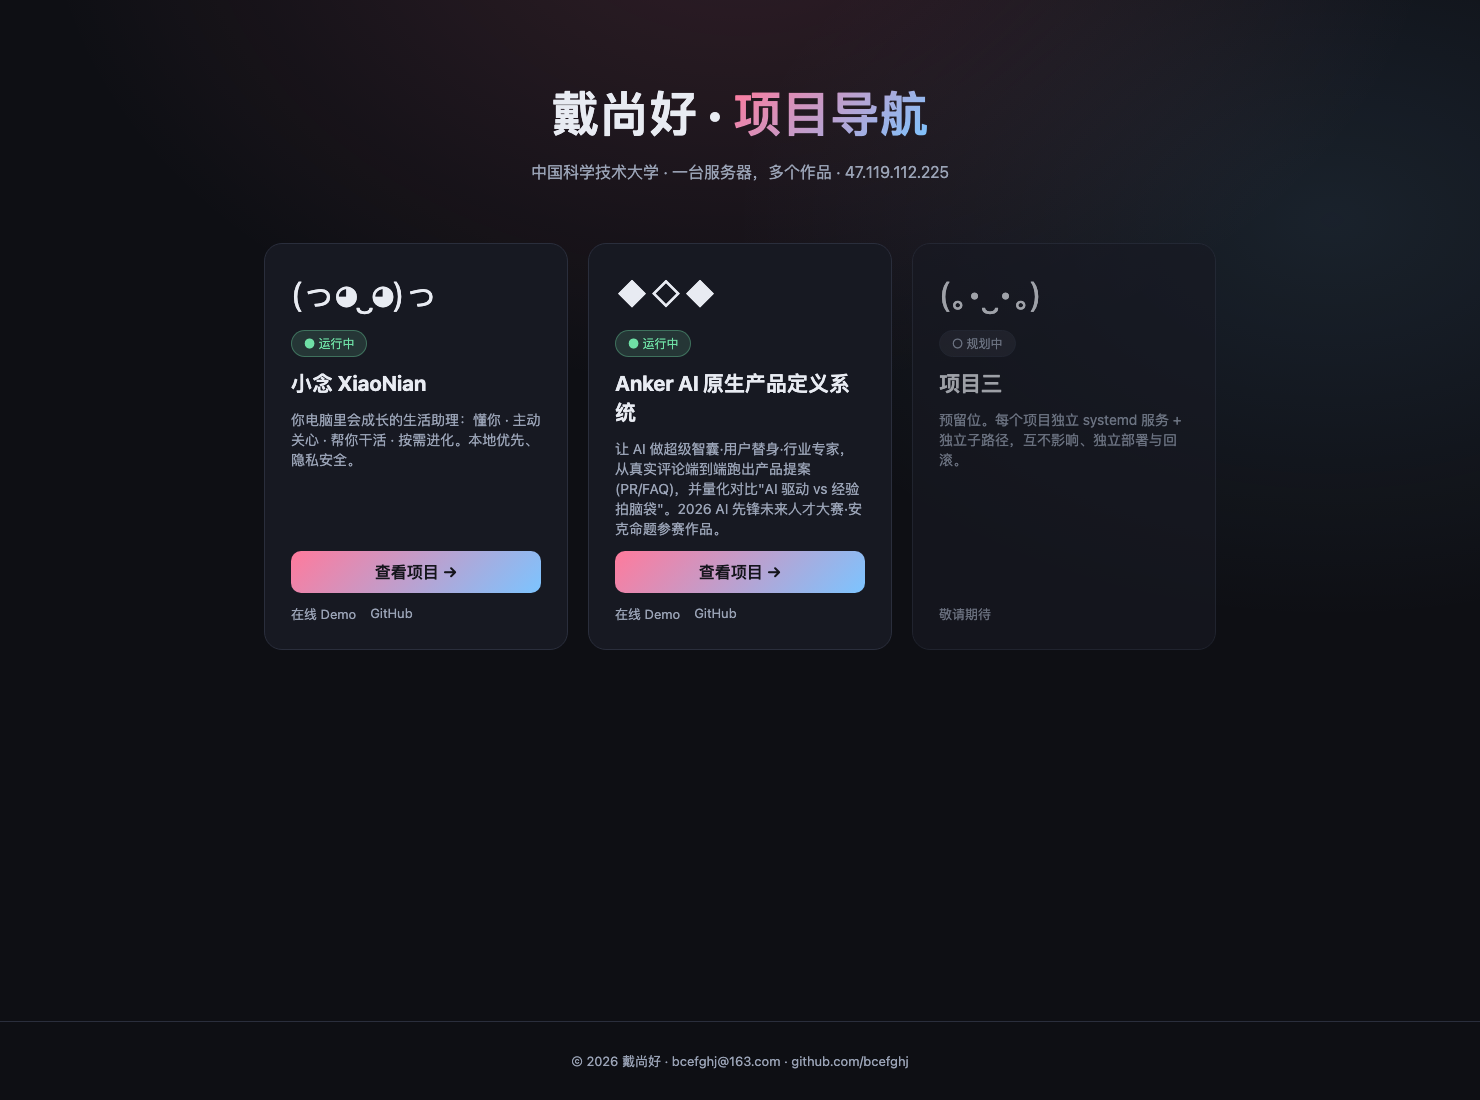
\includegraphics[width=0.92\linewidth]{../figures/hub.png}
\captionof{figure}{项目导航 hub：小念与 Anker 两个作品均"运行中"，互不冲突}
\end{center}

\section{回滚}
停止并禁用 \texttt{anker.service}、注释 nginx 中 anker 的 location、\texttt{nginx -t \&\& systemctl reload nginx} 即可；
小念的服务与路由完全不受影响。
